%************************************************
\chapter[Appendix 4.1: Chapter 4 - Supplementary results]{Appendix 4.1: Chapter 4 - Supplementary results}\label{ch:SAD_appendix}
%************************************************
\renewcommand{\thefigure}{A.4.1.\arabic{figure}}
\setcounter{figure}{0}

\renewcommand{\thetable}{A.4.1.\arabic{table}}
\setcounter{table}{0}

\section*{Supplementary tables}

\begin{table}[ht!]
\centering
\caption[Guild pairs differences in evenness]{\color{Gray}Differences in evenness between pairs of trophic guilds in the empirical datasets, as given by the beta regression detailed in \cref{tab:tab4.3} of chapter 4.}\label{tab:tabApp4.1.4}
\begin{tabular}{llllll}
\hline
contrast  &                       Estimate       & Std. Error & df & z ratio & p-value \\
\hline
plants - herbivores    & -0.868 & 0.054 & Inf & -15.882 &  $<0.05$ \\
plants - omnivores    &  -0.753 & 0.063 & Inf & -11.975 & $<0.05$ \\
plants - carnivores   &  -0.712 & 0.069 & Inf & -10.382 & $<0.05$ \\
herbivores - omnivores &  0.115 & 0.05 & Inf &  2.315 & 0.0947 \\
herbivores - carnivores & 0.157 & 0.061 & Inf &  2.567 &  0.0503 \\
omnivores - carnivores  & 0.042 & 0.068 & Inf &  0.614 & 0.927 \\
\hline
\end{tabular}

\end{table}

\begin{table}[ht!]
\centering
\caption[Guild pairs differences in skewness]{\color{Gray}Differences in skewness between pairs of trophic guilds in the empirical datasets, as given by the multinomial regression detailed in \cref{tab:tab4.2} of chapter 4.}\label{tab:tabApp4.1.5}
\begin{tabular}{llllll}
\hline
contrast  &                       Estimate       & Std. Error & df & t ratio & p-value \\
\hline
category = [-0.5,0.5]: & & & & & \\
plants - herbivores    & -0.216 & 0.066 & 10 & -3.269 & $<0.05$ \\
plants - omnivores     & -0.343 & 0.072 & 10 & -4.761 & $<0.05$ \\
plants - carnivores    & -0.205 & 0.078 & 10 & -2.623 & $<0.05$ \\
herbivores - omnivores & -0.126 & 0.047 & 10 & -2.666 & 0.0930 \\
herbivores - carnivores &  0.011 & 0.053 & 10 &  0.215 & 0.9963 \\
omnivores - carnivores  & 0.138 & 0.063 & 10 &  2.195 & 0.1898 \\

category = (0.5,1]: & & & & & \\
plants - herbivores    &  0.216 & 0.066 & 10 &  3.269 & $<0.05$ \\
plants - omnivores     &  0.343 & 0.072 & 10 &  4.762 & $<0.05$ \\
plants - carnivores    &  0.205 & 0.078 & 10 &  2.623 & 0.0994 \\
herbivores - omnivores &  0.127 & 0.047 & 10 &  2.666 & 0.0930 \\
herbivores - carnivores & -0.011 & 0.053 & 10 & -0.215 & 0.9963 \\
omnivores - carnivores & -0.138 & 0.063 & 10 & -2.195 & 0.1899 \\

category = [-1,-0.5): & & & & & \\
plants - herbivores    & $-5.4*10^{-6}$ & $3*10^{-5}$ & 10 & -0.179 & 0.9978 \\
plants - omnivores     & $-2.8*10^{-6}$ & $1.6*10^{-5}$ & 10 & -0.174 & 0.9980 \\
plants - carnivores    & $-1.8*10^{-5}$ & $1*10^{-4}$ & 10 & -0.178 & 0.9979 \\
herbivores - omnivores &  $2.6*10^{-6}$ & $1.5*10^{-5}$ & 10 &  0.176 & 0.9979 \\
herbivores - carnivores & $-1.3*10^{-5}$ & $7.4*10^{-5}$ & 10 & -0.177 & 0.9979 \\
omnivores - carnivores & $-1.5*10^{-5}$ & $8.8*10^{-5}$ & 10 &  -0.178 & 0.9979 \\
\hline
\end{tabular}

\end{table}

\begin{table}[ht!]
\centering
\caption[Guild species/individuals]{\color{Gray}Differences between the proportion of species and individuals of the mammal trophic guilds, analyzed via Wilcoxon signed-rank paired tests.}\label{tab:tabApp4.1.6}
\begin{tabular}{lllllll}
\hline
  trophic guild  & mean sp &  s.d. sp & mean ind & s.d. ind & W & p-value \\
\hline
herbivores       &    0.623   &   0.216   &      0.607  &     0.324 &  131422 & 0.144 \\
omnivores        &    0.330   &   0.198   &      0.408  &     0.313 &  162226 & $<0.05$ \\
carnivores       &    0.305   &   0.179   &      0.211  &     0.244 &   18772 & $<0.05$ \\
\hline
\end{tabular}

\end{table}

\clearpage

\subsection*{Supplementary figures}

\begin{figure}[ht!]
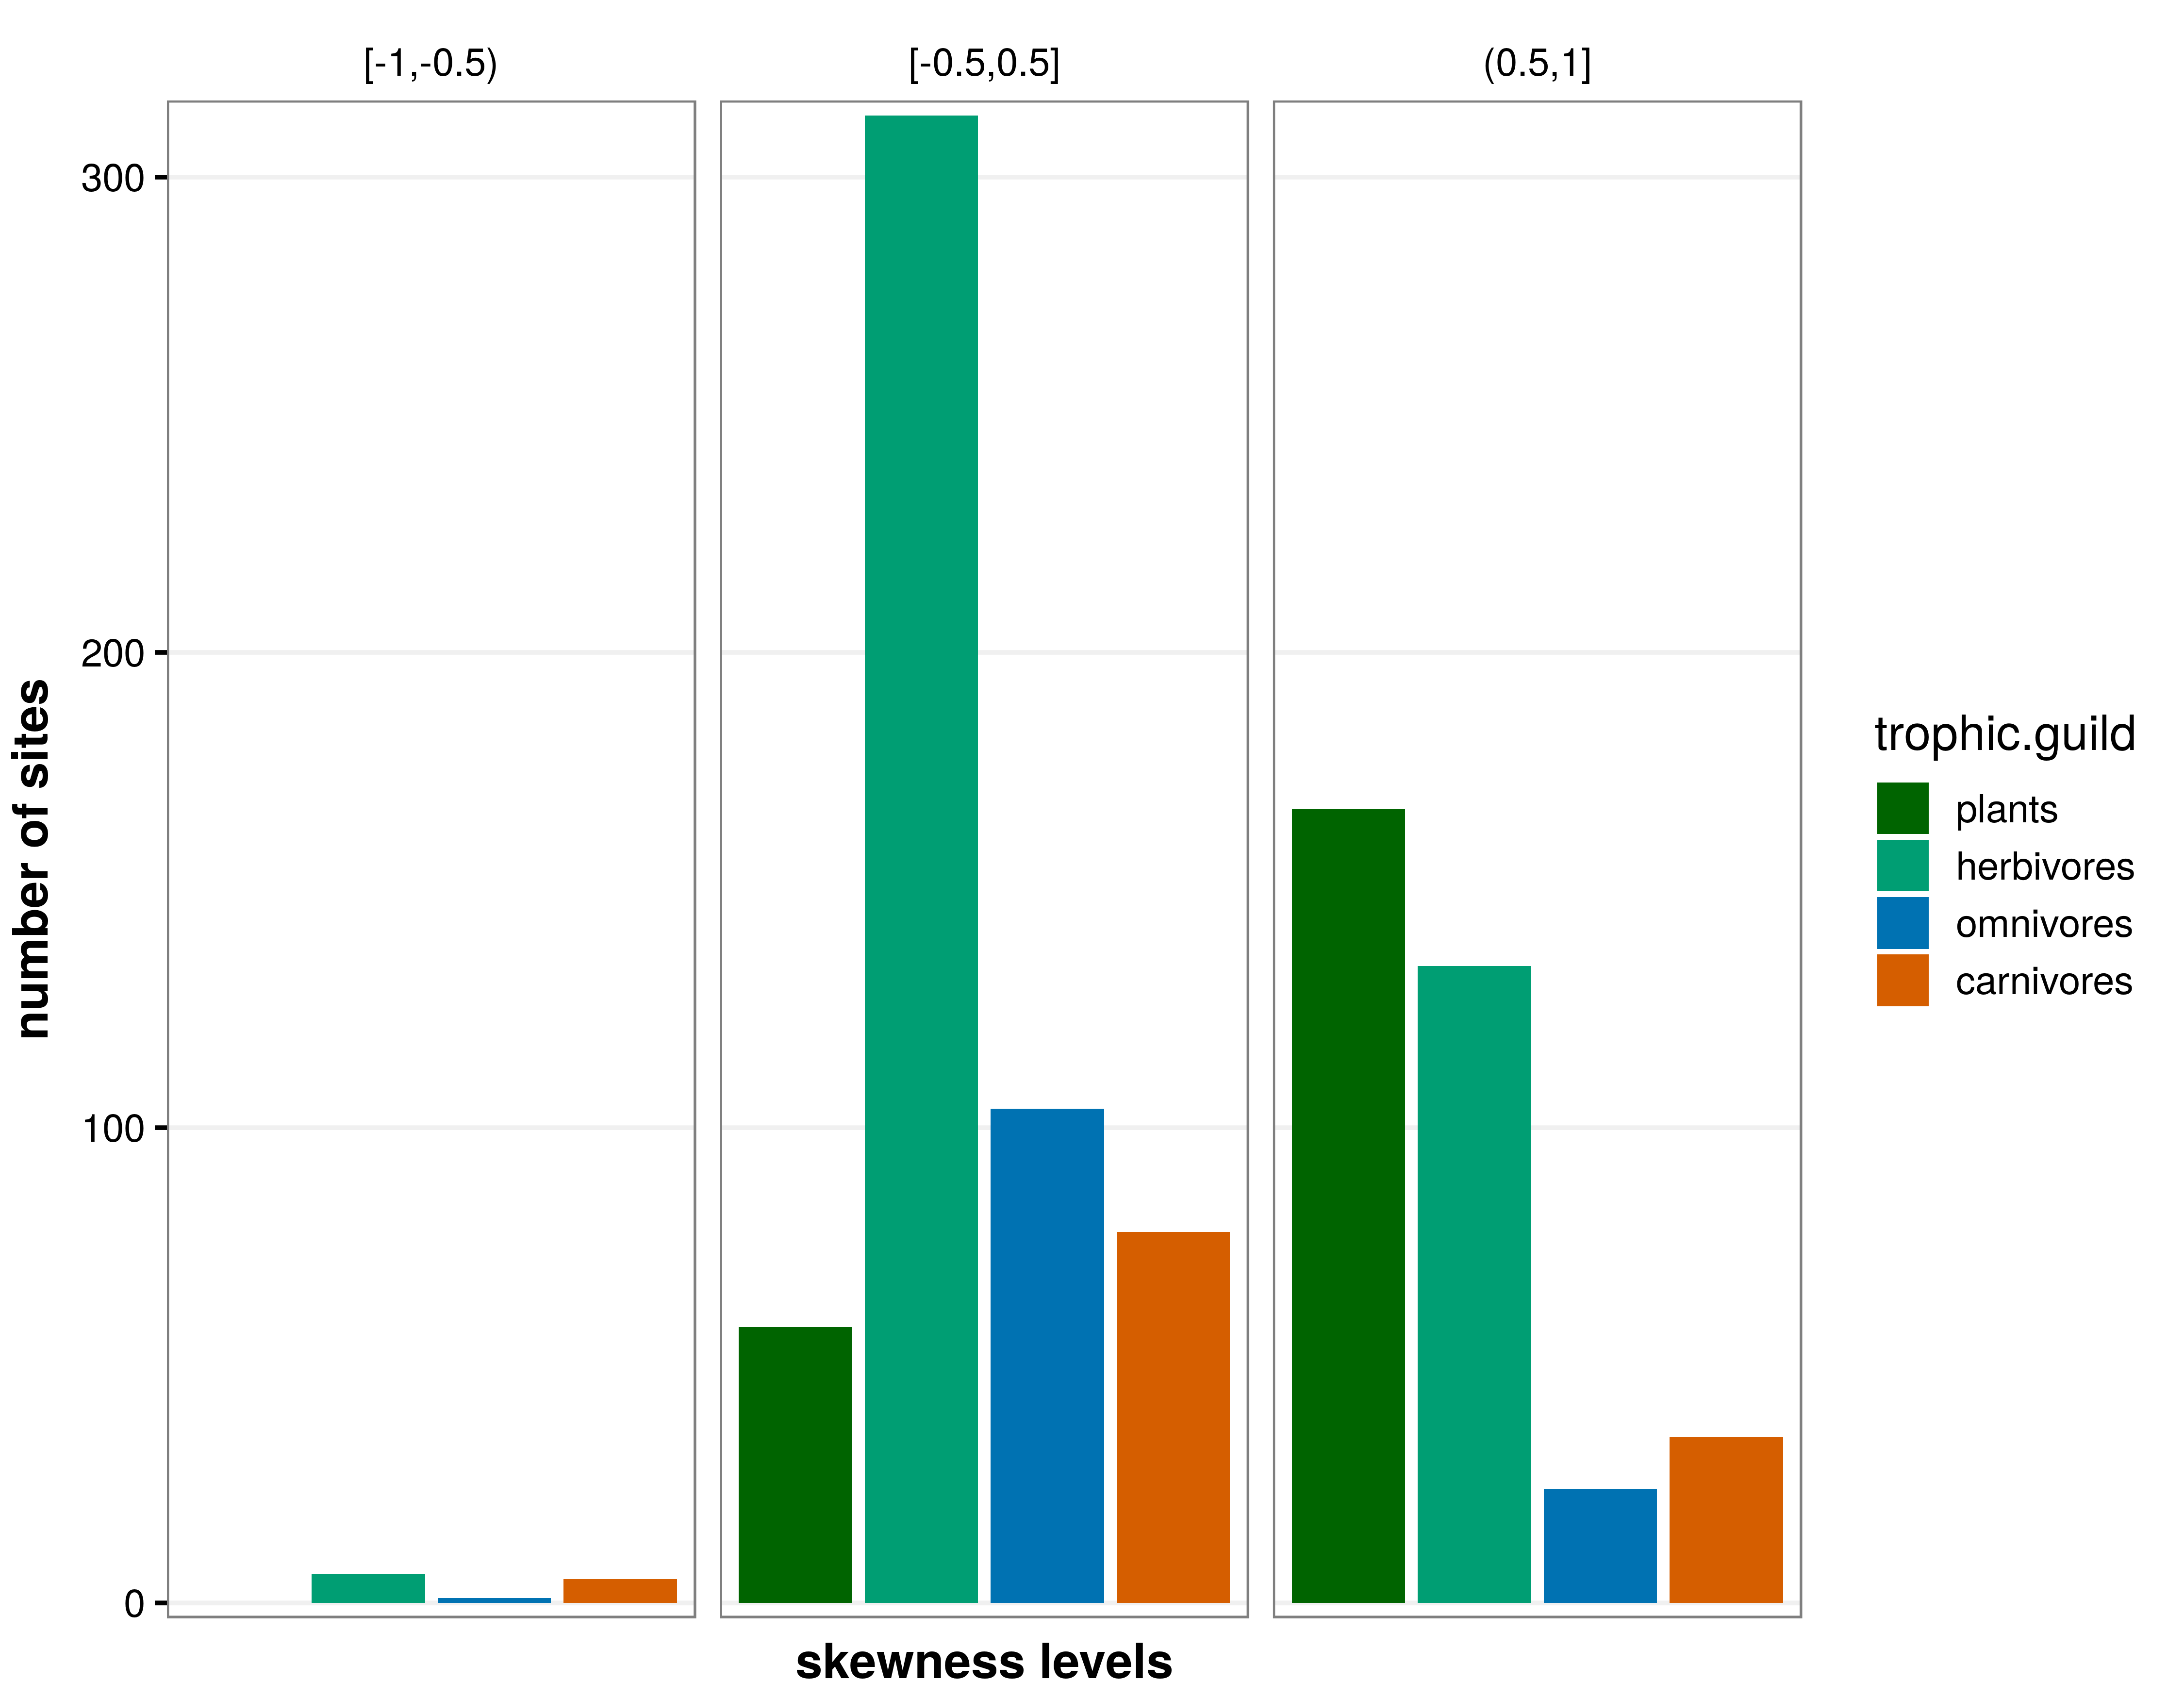
\includegraphics[width=\textwidth,height=\textheight,keepaspectratio]{./Figures/Appendix4_1/Fig_5.png}
\caption[Observed skewness levels]{\color{Gray}Skewness levels observed in empirical datasets}\label{fig:figApp4.1.5}
\end{figure}
